% !TeX program = xelatex
\documentclass{article}
\usepackage{iclr2026_conference,times}

\usepackage{fontspec}
\usepackage{xeCJK}
\setCJKmainfont[
  Path=fonts/,
  BoldFont=NotoSerifCJKsc-Bold.otf
]{NotoSerifCJKsc-Regular.otf}

\usepackage{graphicx}
\usepackage{float}
\usepackage{amssymb}
\usepackage{amsmath}
\usepackage{booktabs}
\usepackage{array}
\usepackage{tabularx}
\usepackage{enumitem}
\usepackage{pifont}
\usepackage{xcolor}
\usepackage{hyperref}
\usepackage{url}
\usepackage{tikz}
\usetikzlibrary{arrows.meta,positioning,calc}

\emergencystretch=1.2em
\setlist{nosep,leftmargin=*}
\setlength{\textfloatsep}{10pt plus 2pt minus 2pt}
\setlength{\dbltextfloatsep}{6pt plus 2pt minus 2pt}
\setlength{\dblfloatsep}{6pt plus 2pt minus 2pt}
\setlength{\abovecaptionskip}{4pt}
\setlength{\belowcaptionskip}{0pt}
% ICLR 模板默认使用 \flushbottom；遇到不可拆分的 [H] 表格时，会把正文块间距
% 过度拉伸。改为 \raggedbottom，使不可避免的余白只留在页尾。
\raggedbottom

\definecolor{auditblue}{HTML}{0077BB}
\definecolor{auditteal}{HTML}{009988}
\definecolor{auditorange}{HTML}{EE7733}

% The Latin lockup uses explicit optical small capitals so M and P remain prominent.
\newcommand{\MuralPresenterLogo}{\mbox{M\raisebox{0.08ex}{\scalebox{0.78}{URAL}}P\raisebox{0.08ex}{\scalebox{0.78}{RESENTER}}}}
\newcommand{\sys}{MuralPresenter}
\newcommand{\fullsys}{\MuralPresenterLogo}
\newcommand{\bench}{ThreadBench}
\hyphenation{ThreadBench}
\newcommand{\tbd}[1]{\textcolor{auditorange}{\textsc{[TBD-#1]}}}
% Preserve unique placeholder IDs in source while keeping result tables readable.
\newcommand{\resulttbd}[1]{\textcolor{auditorange}{\textsc{TBD}}}
\newcommand{\pilot}[1]{\textcolor{auditteal}{\textsc{#1}}}

\title{\fullsys: Multi-Agent Unified\\
Reasoning and Authoring for Long-Horizon\\
Presentations}

\author{Anonymous authors \\ Paper under double-blind review}

%\iclrfinalcopy
\begin{document}

\maketitle
\vspace{-0.5em}

% Generated mechanically from the reviewed Markdown source.
% Controller edits should be made in both source and LaTeX when material.

\begin{abstract}

一张幻灯片可以局部正确却与整册矛盾：前页定义的术语在远处被改写，视觉编码反转，或数值前提被引用却从未建立。这类失败源于创作决策跨阶段、跨页持续，而执行上下文并不持续。因此，缺失的设计变量是责任粒度：哪些页面必须由同一主体共同负责。\textbf{MuralPresenter} 外置持久整册状态，将制作委派给依赖对齐、互不重叠的 slide group，每组由同一 Group Agent 联合生成、渲染与修改。四阶段工作流依次完成内容接地、冻结整册计划、并行的分组制作与整册复审。配套数据管线向三条 Query Track 注入 Style profile 和任务条件化的长程依赖，再将依赖编译为轨迹过滤的 checklist。我们以 1,000 条经质量控制的轨迹训练 MuralPresenter-9B，并以更大的异构队列训练 MuralPresenter-27B；同时提出 \textbf{ThreadBench}，分开评估中间过程证据与最终制品质量。在 PresentBench 上，MuralPresenter-9B 与 MuralPresenter-27B 的 Overall 分别为 \resulttbd{[TBD:ABS\_M9\_PB]} 和 \resulttbd{[TBD:ABS\_M27\_PB]}；在 ThreadBench 上，二者 Final 分别为 \resulttbd{[TBD:ABS\_M9\_THREAD]} 和 \resulttbd{[TBD:ABS\_M27\_THREAD]}。受控消融进一步表明 \resulttbd{[TBD:ABS\_ABLATION\_SUMMARY]}。这些结果说明，显式责任与可审计交接能支撑长程演示创作。

\end{abstract}

\section{Introduction}

演示文稿是持久决策对象。作者固定术语、选定颜色编码、设定数值前提并建立叙事弧——均在生产之前完成。这些决策在远处的页面上被消费，并在跨版本修改中被重新审视 \citep{maheshwari-etal-2024-presentations,zheng2025pptagent,xu-etal-2025-pregenie}。当消费出错，单页看似成立却与全局矛盾：现有评测已揭示要求遗漏、无依据陈述、数值错误与跨页不一致 \citep{chen2026presentbench}。

这种持久性带来两难。单 Agent 保留统一上下文，却不断累积执行产物，逐步削弱对早期决策的利用 \citep{sun2025contextfolding}。按阶段或逐页拆分隔离了子任务却割裂了责任；拆分能否带来收益取决于任务结构、信息共享与验证位置——而非 Agent 数量 \citep{kim2025scalingagents}。两种极端都未触及关键问题：哪些页面应共同承担一条依赖？

\textbf{MuralPresenter} 以 \textbf{slide group} 作答。Orchestrator 按叙事目的、设计亲缘与跨页依赖，把全部页面划入完整且不重叠的组。同一 Group Agent 生成、检查并修改组内所有页面；独立组并行执行；整册 Review 兜底跨组关系。持久状态被外置，使每个阶段读取投影而非原始历史；确定性的解析、下载、渲染与构建始终作为工具。Figure~\ref{fig:page-topologies} 对比此拓扑与顺序、逐页方案。HTML 是创作源，图片、PDF 与 PPTX 转换属于交付边界。

\begin{figure*}[t]
\centering
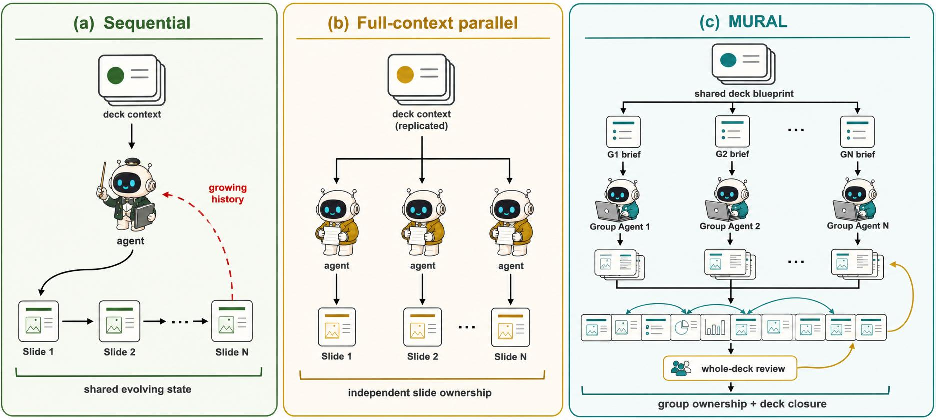
\includegraphics[width=0.90\textwidth]{figures/fig1_page_topologies.pdf}
\caption{\textbf{三种页面生产拓扑及其责任边界。}
顺序式生成保留一段持续增长的历史；full-context parallel 将相同 deck context 交给逐页
worker。\sys{} 外置共享状态，编译依赖对齐的页面组，并由同一 Group Agent 联合生成和检查
整组页面。因此组内关系拥有共同责任主体，剩余跨组关系由 whole-deck Review 处理。}
\label{fig:page-topologies}
\end{figure*}


定义 slide group 的依赖同样支配训练任务构造。三条 Query Track 汇入共享增强层，由该层统一注入 Style、构造与任务匹配的长程依赖并编译成 QC checklist；候选轨迹据此接受过滤。我们以受控的 1K 轨迹语料训练 MuralPresenter-9B，并以六个经质量控制与重加权的异构历史批次训练 MuralPresenter-27B（§4）。\textbf{ThreadBench}（Tracing Handoffs, Requirements, and Execution Across Deck Generation）评价过程–制品一致性，并在 Final Deck rubric 中包含跨页语义一致性；PresentBench 与 SlidesGen-Bench 补充通用质量，DECKBench 评估多轮修改。本文贡献如下：

\begin{enumerate}
\item \textbf{覆盖完整生命周期的 Skill 驱动框架}，明确划分确定性工具与隔离 Agent 上下文。
\item \textbf{依赖对齐的责任拓扑}，由同一 Group Agent 联合负责相关页面，修改仅按必要范围重放。
\item \textbf{可控合成管线与两个已训练模型}：MuralPresenter-9B 使用三 Track 构造的 1,000 条 post-QC 轨迹，MuralPresenter-27B 使用六个经质量控制的历史批次。
\item \textbf{ThreadBench}：面向中间交接与最终 deck 质量的 process-aware、artifact-grounded 评测，并与通用生成、多轮修改 benchmark 配套。
\end{enumerate}

后续结构如下：§2 综述相关工作，§§3–4 介绍创作系统与数据管线，§§5–6 定义 ThreadBench 与评测协议，§§7–8 通过可追踪案例、有效性边界与结论收束全文。

\section{Related Work}

\textbf{演示文稿生成。} 内容选择方法关注每页应放什么 \citep{bandyopadhyay-etal-2024-enhancing-presentation,maheshwari-etal-2024-presentations}；Agent 系统进一步引入整册规划 \citep{zheng2025pptagent}、基于渲染的复审 \citep{xu-etal-2025-pregenie}、专门角色 \citep{xie2026slidebot}、迭代视觉优化 \citep{zheng2026deeppresenter}、讲稿联合与交付 \citep{yang2026deepslide}，以及设计–代码解耦 \citep{cui2026designfirst}。讲稿联合与交付支持属既有工作；MuralPresenter 的区分点在于以 slide group 归属跨页 source-to-target 关系。

\textbf{长程状态与 Agent 粒度。} 增长的历史在上下文窗口耗尽之前已妨碍对早期信息的利用 \citep{sun2025contextfolding}；外置已验证状态并使用新鲜上下文可稳定长轨迹 \citep{ma2026longhorizonharness}。由于拆分收益取决于任务结构与信息流 \citep{kim2025scalingagents}，MuralPresenter 按依赖结构而非流水线阶段或页面序号划定组边界。

\textbf{Agentic 数据与优化。} 完整交互轨迹保留规划决策与工具使用 \citep{zeng2023agenttuning,chen2024agentflan}，迭代反馈教授诊断与修复 \citep{madaan2023selfrefine}。MuralPresenter 依据 rollout 前注入的可机核依赖接收轨迹，并以受控消融检验 inspect–diagnose–patch 轨迹能否迁移到修改任务。

\textbf{评测基准。} PresentBench 评估材料接地生成 \citep{chen2026presentbench}；SlidesGen-Bench 覆盖 Content、Aesthetics 与静态 Editability \citep{yang2026slidesgenbench}；DECKBench 研究生成与多轮修改 \citep{jang2026deckbench}。PPTArena 与 PPT-Eval 检验复合或 PowerPoint 原生修改 \citep{ofengenden2025pptarena,gandhi2026ppteval}，LH-Bench 以 Skill 接地 rubric 评价过程与输出 \citep{gupta2026lhbench}。ThreadBench 将 case-specific 的 Research、Planning、Image 与 Slide-production 证据同 Knowledge、Deck 和 Page 质量分开评分，补充仅看最终产物的评测。

% Generated mechanically from the reviewed Markdown source.
% Controller edits should be made in both source and LaTeX when material.

\section{MuralPresenter}

Figure~\ref{fig:release-workflow} 给出系统总览。MuralPresenter 先外置任务与整册状态，再仅把能独立交付与验收的工作交给新鲜 Agent 上下文，将存在依赖的页面绑定给共享 Group Agent，最后以渲染接地的整册复审闭合剩余关系。§§3.1–3.3 依次形式化任务与状态投影、规定角色边界，并定义分组、视觉批判与按范围修改。

\subsection{长程演示创作任务}

我们把演示文稿创作建模为一个交互式智能体任务。给定用户请求 \(q\)、可选附件 \(\mathcal{M}\)、语言 \(\ell\) 与目标页数 \(N\)，系统在工具库 \(\mathcal{T}\) 与持久状态 \(\mathcal{S}\) 构成的环境中运行，产出演示文稿 \(D=(s_1,\ldots,s_N)\) 连同逐页讲稿与渲染结果。

生成过程是一条多步轨迹 \(\tau\)，按创作生命周期分解为四个阶段： \[
\tau \;=\; \tau^{\mathrm{ground}} \circ \tau^{\mathrm{plan}} \circ \tau^{\mathrm{gen}} \circ \tau^{\mathrm{review}},
\] 分别对应内容接地、整册规划、分组生成与整册复审。前一阶段的输出未在 \(\mathcal{S}\) 中就绪时，依赖它的下游不启动；生成阶段进一步分解为并行的页面组轨迹 \(\tau^{\mathrm{gen}}=\{\tau^{G_1},\ldots,\tau^{G_m}\}\)，其中 \(\{G_1,\ldots,G_m\}\) 是 \(\{1,\ldots,N\}\) 的完整划分（§3.3）。

状态外化为上述阶段排序提供依据。每个被接受的产物 \(d\) 以固定的产生阶段与归属角色进入 \(\mathcal{S}\)。角色 \(r\) 只读取其声明的投影： \[
\pi_r(\mathcal{S}) \;\triangleq\; \{d \in \mathcal{S} \mid d \text{ 属于 } r\text{ 声明的读集}\},
\] 模型生成的写入仅面向其声明的写集。在实现中，\(\mathcal{S}\) 对应 deck 持久状态目录，每个 Skill 的角色卡声明 \(\pi_r\)，委派拓扑决定新上下文接收哪些产物；确定性脚本仍可代任何角色派生或更新共享状态。因此，该投影形式化的是委派契约——每个角色负责读取和产出什么——而非硬性文件系统隔离。

该任务是\textbf{长程}的：开篇主线须在结尾回收，前文定义的术语与视觉编码须在后续沿用。我们把这种关系记为跨页依赖 \(g_k=(a_k,T_k,\Phi_k)\)：源页面 \(a_k\) 建立决策，目标集合 \(T_k\) 消费它，判据 \(\Phi_k\) 检验关系是否成立。整册一致性由这些依赖是否闭合来刻画（§5）；MuralPresenter 的设计核心在于在哪些生命周期边界让哪些角色对跨页依赖共同负责。

\subsection{Skill 驱动的多 Agent 协作}

MuralPresenter 把职责表达为可插拔的 Skill，规定每个角色何时触发、读取哪部分状态投影、产出什么以及交回的判据。是否为一项工作单独开 Agent，取决于该工作能否被单独交付与验收；达不到门槛时，Orchestrator 直接以工具完成。

\textbf{Orchestrator.} 贯穿全程，解析用户意图、协调接地、规划整册、委派生产并验收结果，但不搜图、不写页面、不判像素。确定性操作（解析、下载、渲染、构建）始终作为工具直接调用。每页讲稿在规划阶段确定，并由确定性步骤在生产启动前编译为统一演讲产物。Group Agent 仅实现已冻结的可见内容契约，不改写讲稿。经渲染接地的整册 Review 后，最终确定性步骤重新同步演讲产物。

\textbf{Material \& Research.} Material 把附件并行解析为结构化摘要；Research 只在外部事实会改变结论时启动核验，两者共同汇成供全局引用的接地知识。无附件且无待核事实时，两者均不出现。

\textbf{Image.} 仅在页面计划确需照片或生成图时启动，将检索、生成、候选比对与像素核查从全局轨迹中隔离。

\textbf{Group Agent.} 每个 Group Agent 负责一个页面组，在有界轨迹 \(\tau^{G_j}\) 内联合生成并检查组内所有页面（§3.3），维护组内关系而无需与其他组协商。互不依赖的组并行执行。

\textbf{Review.} 生成汇合后，未参与生成的 Review 在隔离上下文中对整册做独立复审，以避免自评偏袒（§3.3）。之后构建工具负责打包与一致性校验。Figure~\ref{fig:release-workflow} 将这些责任边界串联为完整的创作、修改与交付生命周期。

\begin{figure*}[t]
\centering
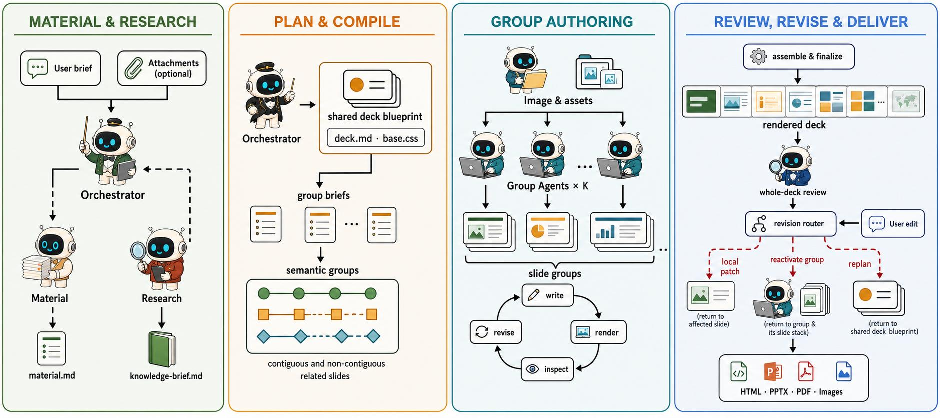
\includegraphics[width=0.90\textwidth]{figures/fig2_release_workflow.pdf}
\caption{\textbf{\sys{} 的完整创作与修改生命周期。}
Material 与 Research 按需接地输入；Orchestrator 写入 blueprint 和 group briefs；Image 准备所需
位图。多个 Group Agent 并行执行 render--inspect--revise，whole-deck Review 检查跨组关系，
revision router 重放最小责任单元。确定性工具负责素材传输、渲染、校验，并封装 HTML、PPTX、
PDF 与图片交付。}
\label{fig:release-workflow}
\end{figure*}


\subsection{分组、视觉批判与修改闭环}

\textbf{依赖对齐的分组。} MuralPresenter 按叙事、设计与素材亲缘，把页面集合划分为完整、不重叠的若干组 \(\{G_1,\ldots,G_m\}\)。整册依赖闭合率分解为： \[
\mathrm{DC}(D)=\underbrace{\frac{1}{K}\!\!\sum_{k:\,\exists j,\,\{a_k\}\cup T_k\subseteq G_j}\!\!\mathbf{1}[\Phi_k\ \text{闭合}]}_{\text{组内，由单一 Group Agent 闭合}}
\;+\;
\underbrace{\frac{1}{K}\!\!\sum_{k:\,\nexists j,\,\{a_k\}\cup T_k\subseteq G_j}\!\!\mathbf{1}[\Phi_k\ \text{闭合}]}_{\text{跨组，由整册复审兜底}}.
\] 分组目标是让尽可能多的强依赖落入组内，只留少数跨组关系给整册复审；组内与跨组闭合的差异在实验中直接测量（§6）。互不依赖的组并行生成。

\textbf{两级视觉批判。} 演示的许多毛病只在渲染时现形。MuralPresenter 把查看渲染像素设为一等操作，分两级执行。组内级：Group Agent 每写一页就渲染、修改，直到页面在像素上成立，再以联系表检查节奏与跨页重复。整册级：Review 在隔离上下文里重看整册渲染；同一独立批判思路也贯穿数据合成（§4）。复审刻意克制：确定性渲染只对 CJK 字体崩坏设硬门，其余信号均作为建议交回。

\textbf{按范围的修改闭环。} 生成后的修改复用同一持久状态。给定一次编辑，路由保守推断影响集 \(I\)：直接触及的页面加上经已知跨页关系牵连的页面。设声明的责任单元为 \(\mathcal{U} = \bigl\{\{i\} \mid i \in [N]\bigr\} \cup \{G_1,\ldots,G_m\} \cup \{[N]\}\)，以包含关系为序；路由策略选择： \[
\mathrm{scope}(I) \;=\; \min_{U \in \mathcal{U}}\; U \quad \text{s.t.} \quad I \subseteq U.
\] 此公式形式化的是已实现的路由策略，而非学习型优化器：系统不保证全局最小代价或完备的依赖知识，影响不明时向更大单元升级。具体而言：单页修改由 Orchestrator 直接处理；触及组内关系则重新激活对应 Group Agent \(\tau^{G_j}\)；需要新事实或素材则按需重启 Research 或 Image；增删页、改动页序或标题链则更新划分并触发整册复审。修改质量与未涉及页面的保持均由多轮实验检验（§6）。最终产物是结构化 HTML，可导出为图片、PDF 与 PPTX。

\section{长程 Agentic 数据合成}

本节介绍数据流水线：任务构建、以外部验证激发反思行为的轨迹合成，以及多阶段过滤（Figure~\ref{fig:data-synthesis}）。下文区分受控的 9B 语料与规模更大的 27B 异构训练队列。

\begin{figure}[H]
\centering
\begin{tikzpicture}
\node[inner sep=0] (datafig) {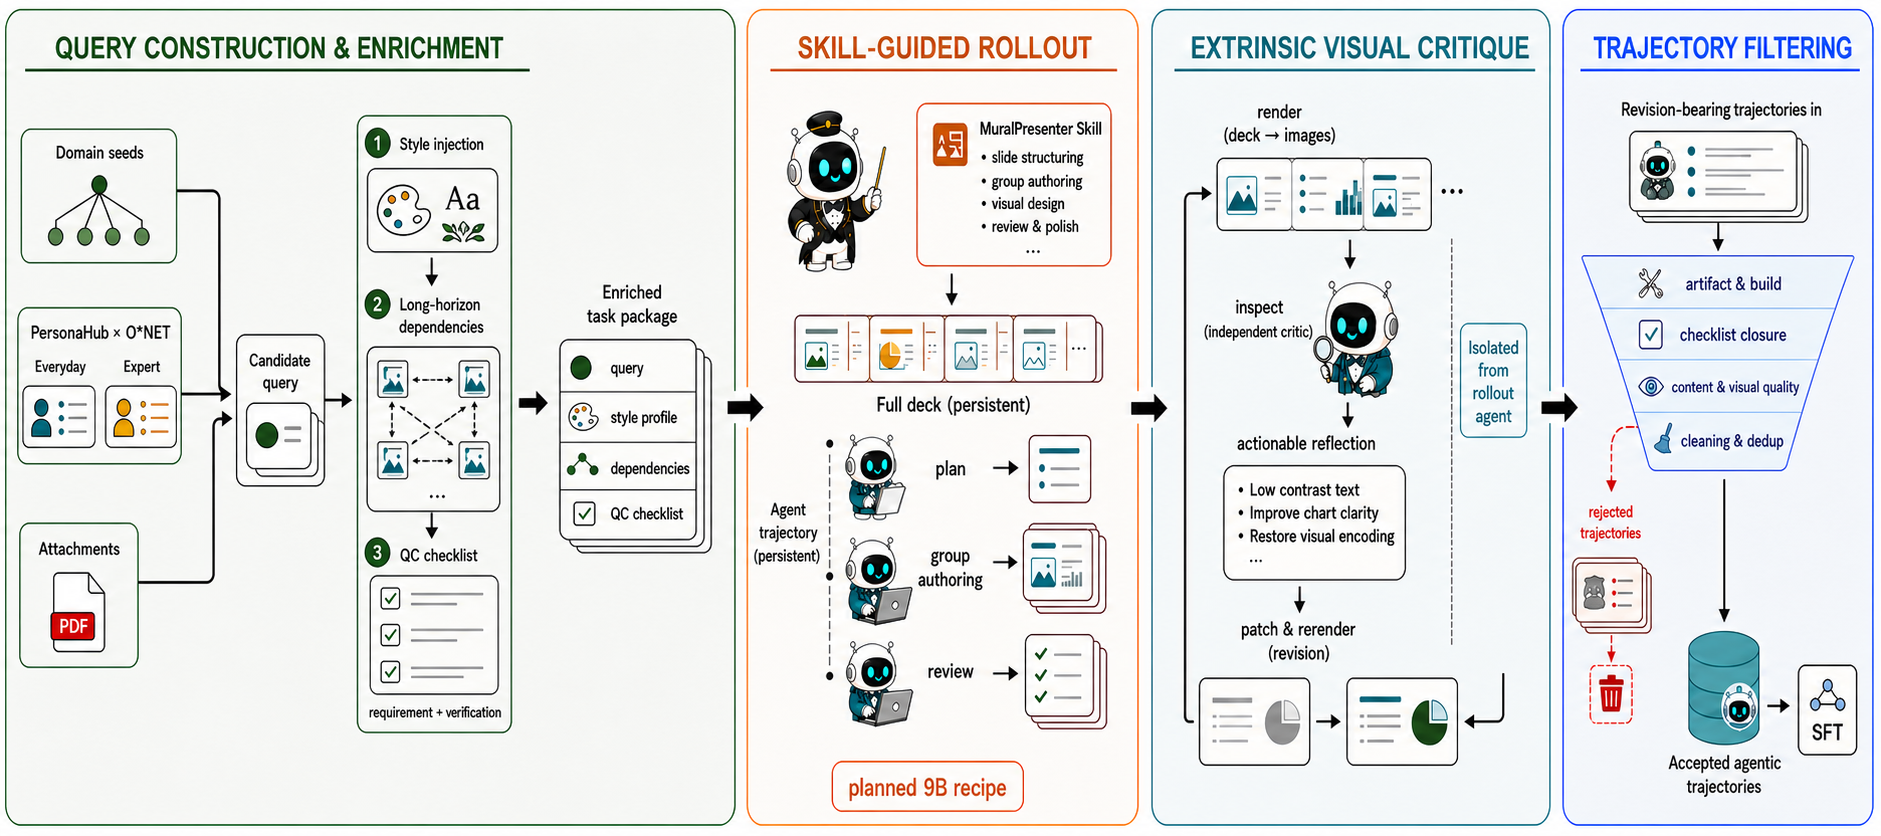
\includegraphics[width=\linewidth]{figures/fig3_long_horizon_agentic_data_synthesis.png}};
\node[fill=white,draw=auditorange,rounded corners=1.5pt,inner xsep=4pt,inner ysep=2pt,font=\scriptsize\sffamily,text=auditorange] at ($(datafig.south west)!0.493!(datafig.south east)+(0,0.43cm)$) {MuralPresenter-9B corpus};
\end{tikzpicture}
\caption{\textbf{长程 Agentic 数据合成。} 三条 Query Track 汇入共享的任务增强层：统一注入 Style profile，构造与任务内容相匹配的长程依赖，并将依赖编译为后续 QC 使用的 checklist。Skill 引导的 rollout 保留规划、分组制作与复审过程；隔离的视觉 critic 以真实渲染触发修改；分层过滤仅保留结构完整且逐项闭合 checklist 的轨迹。该受控管线产出 MuralPresenter-9B 语料；27B 队列具有不同的教师来源与数据规模。}
\label{fig:data-synthesis}
\end{figure}

\subsection{Query 构建}

高质量长程训练要求任务在整册范围内具有可检查的结构。对于 MuralPresenter-9B，我们先从三条互补 Track 构造候选 query，再进入共享的任务增强层。系统从统一风格 taxonomy 中采样 Style profile，将主色、字体气质、装饰母题与留白策略等具体指令织入需求；随后根据任务内容构造长程依赖，包括分节配额、叙事承接、跨页数值一致、视觉母题延续、首尾闭环与显式跨页引用等。本文不以固定数量的约束定义长程性：每项依赖均保留类型、具体要求和闭合条件，并进一步编译成一条 \texttt{longhorizon\_checklist}，同时写明具体要求与后续 QC 的核验方法。

\textbf{Track 1：领域种子扩展。} 从层级化领域池出发，扩展出覆盖广泛学科与场景的任务，侧重广度与多样性。

\textbf{Track 2：人格驱动的真实场景（PersonaHub \(\times\) O*NET）。} 按 O*NET 职业体系匹配演讲者人格并生成 query，分两档：日常通用场景与专家精英场景，后者带有更强领域深度与更长依赖跨度。试点从 84 条初始组合出发，清洗后保留覆盖 65 个职业的 82 条，其中 20 条形成端到端 query。

\textbf{Track 3：附件驱动的反向合成。} 该 Track 从真实文档反向构造"带附件"任务，要求系统接地、引用与重组材料。

三条 Track 合流后，共用同一套 Style taxonomy、输出 schema、长程依赖表示、checklist 编译器与去重策略。最终任务包同时包含面向用户的 query、注入后的 Style profile、显式长程依赖及其 QC checklist；rollout 与过滤因此沿用同一份依赖合约，而不在生成结束后重新猜测验收条件。

\subsection{Skill 引导的轨迹合成}

给定任务，教师模型在与 §3 完全相同的 MuralPresenter 流程下自主生成整套演示，把规划、委派、渲染检查、诊断、补丁与重渲全部保留在轨迹里——监督对象是完整的可执行创作过程，而非仅仅是最终 HTML。

为避免自我验证偏差，我们引入外部验证：独立视觉 critic 在隔离上下文中评判渲染产物，指出溢出、破图、低对比等像素级缺陷，并给出可执行的修改建议注入轨迹。由此，轨迹便带有以真实观察为依据的反思行为。

\textbf{受控的 9B 语料。} 为检验小规模、可明确复现的轨迹数据能否教授完整工作流，我们构建受控实验。DeepSeek-V4-Flash 执行创作流程作为 rollout 主模型，Gemini-3.5-Flash 基于渲染结果提供视觉批判。经确定性校验与质量过滤后，从 \resulttbd{[TBD:9B\_TASKS]} 个任务中保留恰好 1,000 条通过 QC 的训练轨迹。我们以 Qwen-3.5-9B 为基座训练 \resulttbd{[TBD:9B\_EPOCH]} 轮，上下文长度为 \resulttbd{[TBD:9B\_CTX]}，使用 \resulttbd{[TBD:9B\_GPU]} GPU，共消耗 \resulttbd{[TBD:9B\_GPUH]} GPU 小时。

\textbf{已核验的 27B 异构队列。} MuralPresenter-27B 通过全参数监督微调获得，训练数据是在同一创作流程下主要由更高能力的闭源前沿教师模型生成、并经质量过滤的完整智能体轨迹。轨迹保留规划、工具调用、渲染检查、诊断、修改与重渲染过程，而非仅保留最终 HTML。受商业保密约束，本文不披露教师模型的具体身份，但完整报告数据处理流程、语料统计、优化配置与训练算力。该队列来自六个异构历史批次，经 QC-v2 过滤后含 17,171 条任务与 304,275 条有效轨迹；其中 16,073 条任务 / 293,846 条轨迹通过结构核验进入 SFT 候选集，剔除异常与不完整样本后保留 293,436 条基础轨迹；经 Mixture-v2 重采样后训练暴露量 318,422 次，内容 token 数 7.3127B，packed 序列数 56,458 条。Gemini-3.5-Flash 在该队列中仅用于事后质量评分，而非 rollout 教师或 critic。该队列不与 9B 目标集共享教师来源。

\subsection{轨迹过滤}

多阶段过滤保证数据质量：确定性检查核验必需产物、页面覆盖、构建与渲染；结构与约束检查逐条核验跨页要求与用户约束；质量评分对内容与视觉一致性打分；轨迹级清洗去除异常、不完整与近重复样本。失败或不可核验的轨迹仍计入统计，但不会被改写为可用数据。我们区分 query、rollout、完成与被接收四类计数，在数据卡中报告各阶段留存与拒绝原因，并在 §6 汇总过滤后规模。

% Generated mechanically from the reviewed Markdown source.
% Controller edits should be made in both source and LaTeX when material.

\section{ThreadBench}

\subsection{过程–制品评测}

一套视觉精美的 deck 可以掩盖断裂的交接：研究证据可能从未进入规划，规划中的图片可能从未使用，渲染中发现的缺陷也可能从未修复。仅看最终页面无法定位在哪一环断裂。ThreadBench 因此把 case-specific 的过程证据与最终 deck 分开评价。它是 process-aware、artifact-grounded benchmark，但不声称覆盖全部工程环节。

\begin{figure}[H]
\centering
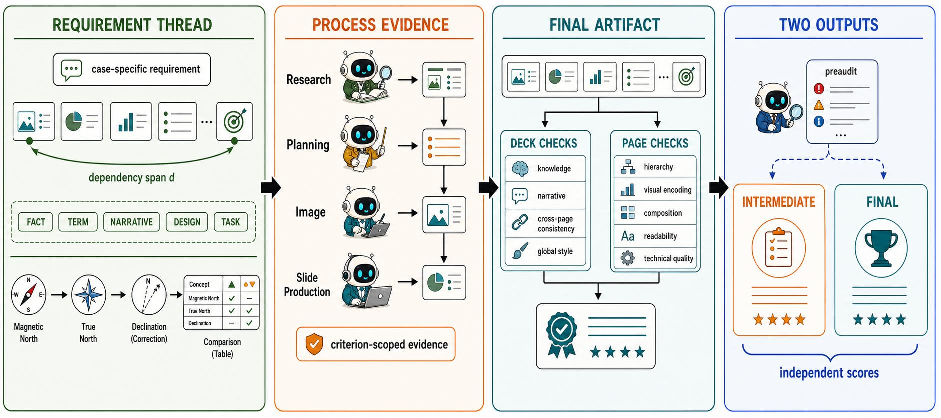
\includegraphics[width=\linewidth]{figures/fig4_threadbench_anatomy.pdf}
\caption{\textbf{ThreadBench 的评测结构。} 每条任务专属需求定义一项跨越整册、可观察的 source-to-target 闭合规则。Intermediate 沿 Research、Planning、Image 与 Slide Production 检查锚定的过程证据；Final 则从整册和逐页两个粒度检查 canonical render。两层分别输出分数，不合并为单一指标。图中的动物导航需求链来自当前正式参考 case。}
\label{fig:threadbench-anatomy}
\end{figure}

\subsection{需求链与双层 Rubric}

Figure~\ref{fig:threadbench-anatomy} 明确了评测单元。需求链从 source requirement 或 anchor 出发，指定远处 target 与可观察的闭合规则，可包含事实、术语、叙事、设计或任务依赖。Intermediate 以 criterion-scoped packet 检查 Research、Planning、Image 和 Slide Production 四个维度下的七类 criterion，每次只暴露与当前单元相关的锚定证据。Final 面向 canonical artifact 分成两组：Deck 将 Knowledge checklist 与六个整册维度结合，Page 则对每个 canonical 页面评价五个视觉与技术维度。完整 criterion 清单和维度定义见附录~\ref{app:protocol}。

\subsection{评分与发布边界}

Judge 先将证据匹配到显式 anchor，再由代码派生 0/0.5/1（Knowledge 为 binary）。Deck 与 Page 各执行一次最弱维度衰减，Intermediate 不衰减：

\[
G_{\mathrm{eff}}=G_{\mathrm{base}}[1-0.3(1-G_{\min})],\quad
F=\tfrac12(Deck_{\mathrm{eff}}+Page_{\mathrm{eff}}),\quad
I=\operatorname{mean}(R,P,I_m,S).
\]

其中 \(I_m\) 表示 Image 维度，Intermediate 只计入适用维度。正式发布的 Intermediate \(I\) 与 Final \(F\) 字段相互独立，不合并为单一标量。当前 v004 可执行合约规定一个正式参考 case（\url{Education/Education-lh-Animal_navigation}）。N/A 语义、major 缺陷扣分、可选且不计分的 Preaudit 及人类–Judge 校准均移至附录~\ref{app:protocol}；多领域扩展与显式 span 诊断不在当前发布范围内。

\section{Experiments}

我们围绕四个研究问题组织实验：\textbf{RQ1（通用质量）} MuralPresenter 生成的完整 deck 在通用质量评测上处于什么水平？\textbf{RQ2（多轮修改）} 在没有专门编辑训练的情况下，它能否完成多轮修改？\textbf{RQ3（过程–制品一致性）} 生产链路是否将需求和证据从中间阶段保持到最终 deck？\textbf{RQ4（设计选择）} 委派边界、责任拓扑、两级视觉批判与轨迹监督各自贡献多少？

\subsection{实验设置}

\textbf{MuralPresenter-9B。} 我们以 DeepSeek-V4-Flash 为 rollout 主模型、Gemini-3.5-Flash 为视觉 critic，在 \resulttbd{[TBD:9B\_TASKS]} 个训练任务上采样轨迹（§4），经质量过滤后保留恰好 1,000 条通过 QC 的训练轨迹。我们使用 MS-SWIFT~\citep{zhao2024mswift} 对 Qwen-3.5-9B 做监督微调：\resulttbd{[TBD:9B\_EPOCH]} 个 epoch、全局批次 32、学习率 \(1\times10^{-5}\)、最大上下文 \resulttbd{[TBD:9B\_CTX]} tokens，并在 \resulttbd{[TBD:9B\_GPU]} 张 A800 上训练 \resulttbd{[TBD:9B\_GPUH]} GPU 小时。

\textbf{数据与训练（已核实的 27B）。} MuralPresenter-27B 使用 §4 所述闭源教师轨迹队列：293{,}436 条基础轨迹经重采样与长度过滤形成 318{,}422 条训练曝光、约 73.1 亿个内容 token 和约 56{,}458 条 128K packed 序列。用 MS-SWIFT 的 Megatron 后端对 Qwen-3.5-27B 做全参数监督微调：上下文 128K、1 个 epoch、全局批次 32、初始学习率 \(2\times10^{-5}\) 经 5\% 线性预热后以余弦策略衰减至 \(1\times10^{-6}\)；4 节点共 32 张 80GB GPU，配置 TP=4、CP=2、DP=4、micro-batch=1、梯度累积 8，冻结视觉编码器与模态对齐器。训练共 1{,}764 个优化步、约 50.3 小时、合计约 1{,}604 GPU 小时。Gemini-3.5-Flash 在此仅作 QC 阶段的质量评分。完整数据与模型台账见附录~\ref{app:protocol}。

\textbf{基线。} ThreadBench 保留六个强通用模型对照：Opus-4.7、Sonnet-5、GPT-5.6-luna、Gemini-3.5-Flash、Qwen-3.7-plus 与 Kimi-k3。已有 benchmark 的重跑采用精简五系统组：9B 合成管线（DeepSeek-V4-Flash + Gemini-3.5-Flash）、未微调 Qwen-3.5-9B 与 Qwen-3.6-27B 对照，以及我们的 9B 和 27B。五者共享同一 benchmark 输入与 adapter。为显示模型在各外部 benchmark 上的绝对位置，Tables~\ref{tab:general}--\ref{tab:edit} 另设 \emph{reported} 分块，列入原论文中的代表性领先系统。这些数值沿用各自来源协议，不是本文重跑结果，也不与统一重跑组混合统计或进入显著性检验；完整 reported 表见附录~\ref{app:protocol}。

\textbf{解释边界。} 9B 与 27B 在教师来源、数据规模、基座模型和训练配方上均不相同，因此二者只作为两种系统配置分别报告，不将分数差异解释为受控的模型扩展或数据效率结论。方法与组件消融（RQ4）在 9B 受控设置下进行，使用同一 1K 语料并固定其余训练变量。ThreadBench 中与闭源前沿系统的对比属端到端系统比较，不构成与教师无关的泛化性证据。

\textbf{评测口径。} PresentBench~\citep{chen2026presentbench} 与 SlidesGen-Bench~\citep{yang2026slidesgenbench} 衡量通用生成质量，DECKBench~\citep{jang2026deckbench} 衡量多轮修改，ThreadBench（§5）通过独立的 Intermediate 和 Final 分数及维度级诊断衡量过程–制品一致性。有界的质量、相似度、成功率与 ThreadBench 分数均按越高越好解读；SlidesGen-Bench PEI 保持为有序的可编辑性等级，带符号的 DECKBench 变化量则保留官方协议的方向，不与绝对质量分数合并。其余缩放与聚合均遵循官方定义；所有运行均冻结并记录指标版本、方向、聚合代码与哈希。完整维度与次要诊断见附录~\ref{app:protocol}。

\subsection{主要结果}

\textbf{通用生成质量（RQ1）。} Table~\ref{tab:general} 将五系统重跑组与原论文中的代表性领先系统并列，报告 PresentBench Overall 及 SlidesGen-Bench Content、Aesthetics 和 Editability（PEI）。完整子维度与 reported 系统见附录~\ref{app:protocol}。该表回答通用 deck 质量水平，不对长程一致性下结论。

\begin{table}[!htbp]
\centering
\small
\caption{RQ1：原论文代表性领先系统（按来源协议 reported）与本文五系统统一重跑在 PresentBench 和 SlidesGen-Bench 上的结果。完整 reported 系统与维度见附录~\ref{app:protocol}。}
\label{tab:general}
\begingroup
\let\texttt\resulttbd
\setlength{\tabcolsep}{4pt}
\begin{tabularx}{\linewidth}{@{}>{\raggedright\arraybackslash}Xcccc@{}}
\toprule
& PresentBench & \multicolumn{3}{c}{SlidesGen-Bench} \\
\cmidrule(lr){2-2}\cmidrule(lr){3-5}
System & Overall & Content & Aesthetics & Editability (PEI) \\
\midrule
\multicolumn{5}{l}{\emph{原论文参考（reported）}} \\
NotebookLM       & 62.5 & 74.21 & 22.82 & L0 \\
Zhipu            & ---  & 88.29 & 22.06 & L2 \\
Skywork-Banana   & ---  & 83.83 & 27.28 & L1 \\
Quark            & ---  & 81.40 & 16.86 & L3 \\
\midrule
\multicolumn{5}{l}{\emph{统一重跑（相同输入与 adapter）}} \\
9B 合成管线 (DS-V4 + Gemini-3.5) & \resulttbd{[TBD:G\_TC\_PB]} & \resulttbd{[TBD:G\_TC\_SGC]} & \resulttbd{[TBD:G\_TC\_SGA]} & \resulttbd{[TBD:G\_TC\_SGE]} \\
Qwen-3.5-9B（未微调）  & \resulttbd{[TBD:G\_Q9\_PB]}  & \resulttbd{[TBD:G\_Q9\_SGC]}  & \resulttbd{[TBD:G\_Q9\_SGA]}  & \resulttbd{[TBD:G\_Q9\_SGE]} \\
Qwen-3.6-27B（未微调） & \resulttbd{[TBD:G\_Q27\_PB]} & \resulttbd{[TBD:G\_Q27\_SGC]} & \resulttbd{[TBD:G\_Q27\_SGA]} & \resulttbd{[TBD:G\_Q27\_SGE]} \\
MuralPresenter-9B  & \resulttbd{[TBD:G\_M9\_PB]}  & \resulttbd{[TBD:G\_M9\_SGC]}  & \resulttbd{[TBD:G\_M9\_SGA]}  & \resulttbd{[TBD:G\_M9\_SGE]} \\
MuralPresenter-27B & \resulttbd{[TBD:G\_M27\_PB]} & \resulttbd{[TBD:G\_M27\_SGC]} & \resulttbd{[TBD:G\_M27\_SGA]} & \resulttbd{[TBD:G\_M27\_SGE]} \\
\bottomrule
\end{tabularx}
\endgroup
\end{table}

Reported 分块把公开前沿锚定为：PresentBench Overall 62.5（NotebookLM）、Content 88.29（Zhipu）、Aesthetics 27.28（Skywork-Banana）和 PEI L3（Quark）。MuralPresenter-9B 的 PresentBench Overall 为 \resulttbd{[TBD:G\_M9\_PB]}，MuralPresenter-27B 为 \resulttbd{[TBD:G\_M27\_PB]}，统一重跑组中的最强对照为 \resulttbd{[TBD:G\_BEST\_CONTROL\_PB]}。在 SlidesGen-Bench 上，两种模型的 Content/Aesthetics/PEI 三元组分别为 \resulttbd{[TBD:G\_M9\_TRIPLE]} 和 \resulttbd{[TBD:G\_M27\_TRIPLE]}。相对 reported 前沿，\resulttbd{[TBD:G\_REPORTED\_COMPARISON]}；在受控重跑组内，结果表明 \resulttbd{[TBD:G\_RQ1\_INTERPRETATION]}。两类比较均不用于推断长程一致性。

\textbf{多轮修改（RQ2）。} Table~\ref{tab:edit} 将同一五系统重跑组与 DECKBench 原论文中的代表性配置并列，报告 Deck Fidelity、Layout Quality、Transition Similarity、\(\Delta\)-DTW 与 \(\Delta\)-Transition Similarity。PPT-Eval~\citep{gandhi2026ppteval} 仍是补充迁移测试，并列出其 reported 领先参考。原论文完整字段见附录~\ref{app:protocol}。inspect--diagnose--patch 行为迁移是一项由 RQ4 检验的假设。

\begin{table}[!htbp]
\centering
\footnotesize
\caption{RQ2：DECKBench 原论文代表性配置与本文五系统统一重跑；PPT-Eval 仅作补充且保持独立协议。完整 reported 字段见附录~\ref{app:protocol}。}
\label{tab:edit}
\begingroup
\let\texttt\resulttbd
\setlength{\tabcolsep}{3pt}
\begin{tabularx}{\linewidth}{@{}>{\raggedright\arraybackslash}Xccccc@{}}
\toprule
& Deck & Slide & Deck & \multicolumn{2}{c}{Multi-turn} \\
\cmidrule(lr){2-2}\cmidrule(lr){3-3}\cmidrule(lr){4-4}\cmidrule(lr){5-6}
System & Fidelity & Layout Q. & Trans.\ Sim. & \(\Delta\)-DTW & \(\Delta\)-Trans.\ Sim. \\
\midrule
\multicolumn{6}{l}{\emph{原论文参考（reported）}} \\
Auto-Slides (GPT-4o) & 0.591 & 0.998 & 0.858 & --- & --- \\
DECKBench (GPT-4o)   & 0.584 & 1.000 & 0.879 & --- & --- \\
GPT-5.1 模拟器 + GPT-5-mini 编辑器 (High) & --- & --- & --- & 0.02278 & 0.03230 \\
Kimi K2 模拟器 + DeepSeek 编辑器 (High)   & --- & --- & --- & 0.01549 & 0.04287 \\
\midrule
\multicolumn{6}{l}{\emph{统一重跑（相同输入与 adapter）}} \\
9B 合成管线 (DS-V4 + Gemini-3.5) & \resulttbd{[TBD:E\_TC\_DFID]} & \resulttbd{[TBD:E\_TC\_SLQ]} & \resulttbd{[TBD:E\_TC\_DTSIM]} & \resulttbd{[TBD:E\_TC\_MDDTW]} & \resulttbd{[TBD:E\_TC\_MDTS]} \\
Qwen-3.5-9B（未微调）  & \resulttbd{[TBD:E\_Q9\_DFID]}  & \resulttbd{[TBD:E\_Q9\_SLQ]}  & \resulttbd{[TBD:E\_Q9\_DTSIM]}  & \resulttbd{[TBD:E\_Q9\_MDDTW]}  & \resulttbd{[TBD:E\_Q9\_MDTS]} \\
Qwen-3.6-27B（未微调） & \resulttbd{[TBD:E\_Q27\_DFID]} & \resulttbd{[TBD:E\_Q27\_SLQ]} & \resulttbd{[TBD:E\_Q27\_DTSIM]} & \resulttbd{[TBD:E\_Q27\_MDDTW]} & \resulttbd{[TBD:E\_Q27\_MDTS]} \\
MuralPresenter-9B  & \resulttbd{[TBD:E\_M9\_DFID]}  & \resulttbd{[TBD:E\_M9\_SLQ]}  & \resulttbd{[TBD:E\_M9\_DTSIM]}  & \resulttbd{[TBD:E\_M9\_MDDTW]}  & \resulttbd{[TBD:E\_M9\_MDTS]} \\
MuralPresenter-27B & \resulttbd{[TBD:E\_M27\_DFID]} & \resulttbd{[TBD:E\_M27\_SLQ]} & \resulttbd{[TBD:E\_M27\_DTSIM]} & \resulttbd{[TBD:E\_M27\_MDDTW]} & \resulttbd{[TBD:E\_M27\_MDTS]} \\
\midrule
\multicolumn{6}{l}{\emph{PPT-Eval（补充，官方口径，不与上表比较）}} \\
& \multicolumn{2}{c}{Success Rate} & \multicolumn{3}{c}{Avg.\ Partial Score} \\
Claude-4.5-Opus（reported） & \multicolumn{2}{c}{45\%} & \multicolumn{3}{c}{57\%} \\
MuralPresenter-27B & \multicolumn{2}{c}{\resulttbd{[TBD:E\_M27\_PESR]}} & \multicolumn{3}{c}{\resulttbd{[TBD:E\_M27\_PEPS]}} \\
\bottomrule
\end{tabularx}
\endgroup
\end{table}

DECKBench reported 分块直接保留真实系统与配置，而不拼接一个虚构的逐指标最优系统：Auto-Slides 给出表中最高 Fidelity，DECKBench（GPT-4o）给出最高 Layout 与 Transition Similarity，两组 High-granularity 模拟器/编辑器配置提供多轮参考。在统一重跑中，相较未微调 Qwen-3.5-9B，MuralPresenter-9B 的 Deck Fidelity 与 Layout Quality 变化为 \resulttbd{[TBD:E\_M9\_SUMMARY]}；相较 27B 对照，MuralPresenter-27B 的对应变化为 \resulttbd{[TBD:E\_M27\_SUMMARY]}。多轮变化量显示 \resulttbd{[TBD:E\_MULTITURN\_INTERPRETATION]}；相对 reported 外部参考，\resulttbd{[TBD:E\_REPORTED\_COMPARISON]}。PPT-Eval 相对 Claude-4.5-Opus 的 45\%/57\% reported 参考得到 \resulttbd{[TBD:E\_PPTEVAL\_INTERPRETATION]}。结合 RQ4，这些结果支持关于 inspect--diagnose--patch 监督迁移的结论：\resulttbd{[TBD:E\_RQ2\_CONCLUSION]}。

\textbf{过程–制品一致性（RQ3）。} Table~\ref{tab:thread} 报告 ThreadBench 的 Intermediate 和 Final 分数及可解释的组级分列（Deck 和 Page 有效分）。二者为 v004 评分合约（§5.3）的两个独立输出。所有系统的维度级诊断见附录~\ref{app:protocol}。

\begin{table}[!htbp]
\centering
\small
\caption{RQ3：ThreadBench 过程–制品一致性。Intermediate 和 Final 为独立 0–1 分；Deck 和 Page 为 Final 两子组经最弱维度衰减后的有效分。}
\label{tab:thread}
\begingroup
\let\texttt\resulttbd
\setlength{\tabcolsep}{5pt}
\begin{tabularx}{\linewidth}{@{}>{\raggedright\arraybackslash}Xcccc@{}}
\toprule
& \multicolumn{1}{c}{Intermediate} & \multicolumn{3}{c}{Final} \\
\cmidrule(lr){2-2}\cmidrule(lr){3-5}
System & Score & Score & Deck\(_{eff}\) & Page\(_{eff}\) \\
\midrule
Opus-4.7            & \resulttbd{[TBD:T\_OP\_INT]}  & \resulttbd{[TBD:T\_OP\_FIN]}  & \resulttbd{[TBD:T\_OP\_DECK]} & \resulttbd{[TBD:T\_OP\_PAGE]} \\
Sonnet-5            & \resulttbd{[TBD:T\_SN\_INT]}  & \resulttbd{[TBD:T\_SN\_FIN]}  & \resulttbd{[TBD:T\_SN\_DECK]} & \resulttbd{[TBD:T\_SN\_PAGE]} \\
GPT-5.6-luna        & \resulttbd{[TBD:T\_LU\_INT]}  & \resulttbd{[TBD:T\_LU\_FIN]}  & \resulttbd{[TBD:T\_LU\_DECK]} & \resulttbd{[TBD:T\_LU\_PAGE]} \\
Gemini-3.5-Flash    & \resulttbd{[TBD:T\_GM\_INT]}  & \resulttbd{[TBD:T\_GM\_FIN]}  & \resulttbd{[TBD:T\_GM\_DECK]} & \resulttbd{[TBD:T\_GM\_PAGE]} \\
Qwen-3.7-plus       & \resulttbd{[TBD:T\_QW\_INT]}  & \resulttbd{[TBD:T\_QW\_FIN]}  & \resulttbd{[TBD:T\_QW\_DECK]} & \resulttbd{[TBD:T\_QW\_PAGE]} \\
Kimi-k3             & \resulttbd{[TBD:T\_KM\_INT]}  & \resulttbd{[TBD:T\_KM\_FIN]}  & \resulttbd{[TBD:T\_KM\_DECK]} & \resulttbd{[TBD:T\_KM\_PAGE]} \\
\midrule
MuralPresenter-9B  & \resulttbd{[TBD:T\_M9\_INT]}  & \resulttbd{[TBD:T\_M9\_FIN]}  & \resulttbd{[TBD:T\_M9\_DECK]} & \resulttbd{[TBD:T\_M9\_PAGE]} \\
MuralPresenter-27B & \resulttbd{[TBD:T\_M27\_INT]} & \resulttbd{[TBD:T\_M27\_FIN]} & \resulttbd{[TBD:T\_M27\_DECK]} & \resulttbd{[TBD:T\_M27\_PAGE]} \\
\bottomrule
\end{tabularx}
\endgroup
\end{table}

MuralPresenter-9B 的 Intermediate/Final 为 \resulttbd{[TBD:T\_M9\_INT]}/\resulttbd{[TBD:T\_M9\_FIN]}，MuralPresenter-27B 为 \resulttbd{[TBD:T\_M27\_INT]}/\resulttbd{[TBD:T\_M27\_FIN]}。相对最强通用基线，两者的对应差值为 \resulttbd{[TBD:T\_M9\_DELTA]} 与 \resulttbd{[TBD:T\_M27\_DELTA]}。Deck/Page 分列进一步显示 \resulttbd{[TBD:T\_RQ3\_INTERPRETATION]}，据此判断主要瓶颈位于需求传递还是最终页面质量。

\subsection{消融（RQ4）}

Table~\ref{tab:ablation} 报告四组单因素 9B 受控实验：使用同一 1K 训练语料并固定其余训练变量，对照同一共享 Full reference。\textbf{委派边界}：单上下文或总是委派。\textbf{责任拓扑}：逐页或固定相邻分组，用于隔离依赖对齐分组相对一般任务拆分的贡献。\textbf{两级视觉批判}：分别移除组内或整册一级。\textbf{轨迹监督}：output-only SFT 或移除 inspect--diagnose--patch 步骤。主要指标为 ThreadBench Intermediate 与 Final，Deck 的跨页语义一致性维度作为拓扑敏感诊断。

\begin{table}[!htbp]
\centering
\footnotesize
\caption{RQ4 受控消融：相对同一 Full reference 单因素比较。Intermediate 与 Final 为聚合输出；Cross-page 为 Final Deck 的跨页语义一致性维度。}
\label{tab:ablation}
\begingroup
\let\texttt\resulttbd
\setlength{\tabcolsep}{3pt}
\begin{tabularx}{\linewidth}{@{}>{\raggedright\arraybackslash}p{0.19\linewidth}>{\raggedright\arraybackslash}Xccc@{}}
\toprule
Factor & Variant & Intermediate & Final & Cross-page \\
\midrule
Full reference (ours) & on-demand + dep.-aligned + both critique + full traj. & \resulttbd{[TBD:A\_FULL\_INT]} & \resulttbd{[TBD:A\_FULL\_FIN]} & \resulttbd{[TBD:A\_FULL\_XSEM]} \\
\midrule
Delegation boundary & Single-context      & \resulttbd{[TBD:A\_DEL\_SC\_INT]}  & \resulttbd{[TBD:A\_DEL\_SC\_FIN]} & \resulttbd{[TBD:A\_DEL\_SC\_XSEM]} \\
                    & Always-delegate     & \resulttbd{[TBD:A\_DEL\_AD\_INT]}  & \resulttbd{[TBD:A\_DEL\_AD\_FIN]} & \resulttbd{[TBD:A\_DEL\_AD\_XSEM]} \\
\midrule
Responsibility topology & Per-slide ownership & \resulttbd{[TBD:A\_TOP\_PS\_INT]}  & \resulttbd{[TBD:A\_TOP\_PS\_FIN]} & \resulttbd{[TBD:A\_TOP\_PS\_XSEM]} \\
                    & Fixed-adjacent      & \resulttbd{[TBD:A\_TOP\_FA\_INT]}  & \resulttbd{[TBD:A\_TOP\_FA\_FIN]} & \resulttbd{[TBD:A\_TOP\_FA\_XSEM]} \\
\midrule
Two-level visual critique & w/o group-level     & \resulttbd{[TBD:A\_VIS\_NG\_INT]}  & \resulttbd{[TBD:A\_VIS\_NG\_FIN]} & \resulttbd{[TBD:A\_VIS\_NG\_XSEM]} \\
                    & w/o whole-deck      & \resulttbd{[TBD:A\_VIS\_NW\_INT]}  & \resulttbd{[TBD:A\_VIS\_NW\_FIN]} & \resulttbd{[TBD:A\_VIS\_NW\_XSEM]} \\
\midrule
Trajectory supervision & Output-only SFT     & \resulttbd{[TBD:A\_SUP\_OO\_INT]}  & \resulttbd{[TBD:A\_SUP\_OO\_FIN]} & \resulttbd{[TBD:A\_SUP\_OO\_XSEM]} \\
                    & w/o inspect--patch  & \resulttbd{[TBD:A\_SUP\_NI\_INT]}  & \resulttbd{[TBD:A\_SUP\_NI\_FIN]} & \resulttbd{[TBD:A\_SUP\_NI\_XSEM]} \\
\bottomrule
\end{tabularx}
\endgroup
\end{table}

将依赖对齐分组替换为逐页或固定相邻责任后，Cross-page 一致性变化为 \resulttbd{[TBD:A\_TOPOLOGY\_EFFECT]}；改变委派边界后，Final 变化为 \resulttbd{[TBD:A\_DELEGATION\_EFFECT]}。移除组内或整册视觉批判得到 \resulttbd{[TBD:A\_CRITIQUE\_EFFECT]}，output-only 与移除 inspect--patch 的监督设置得到 \resulttbd{[TBD:A\_SUPERVISION\_EFFECT]}。组合结果形成结论 \resulttbd{[TBD:A\_RQ4\_INTERPRETATION]}，从而将责任拓扑效应与一般多 Agent 拆分区分开。

% Generated mechanically from the reviewed Markdown source.
% Controller edits should be made in both source and LaTeX when material.

\section{案例分析：追踪动物导航演示中的需求链}

ThreadBench 的正式参考 case 要求制作一套动物导航科学教学演示，同时覆盖地磁、太阳和星辰罗盘的机制说明、科学示意图、真实图片及一个严格的六列三行对比表。这些约束形成一条长程需求链：研究阶段建立的证据要穿过逐页规划与机制讲解，最后在统一口径下进入对比表。Research 记录证据与术语，Orchestrator 将需求投影到整册和逐页合约及图片任务，Group Agent 联合制作相关的机制页与综合页，整册 Review 再检查末尾对比是否延续前文概念。持久产物因而暴露三段可检查的交接：证据进入计划，计划与资产进入页面，页面组汇入最终整册。

任务专属 rubric 进一步定位在成品中看似相似的失效：机制证据缺失属于 Research，正确证据未进入逐页合约属于 Planning，资产未使用或页面未经渲染检查属于制作阶段；即使中间产物齐全，对比维度错误、术语不一致或视觉编码不可读仍属于最终成品失败。这种分离既给实践者具体修复目标，也避免以“流程完成”代替成品质量。本文将该 case 用作定性追踪，而由受控 9B 消融承担责任拓扑的因果检验。证据边界仍然明确：9B 与 27B 在数据和训练上存在混杂，LLM 判定受其与人工评分的一致性上限约束，当前 benchmark 仅有一个正式 case，而 HTML 到 PDF/PPTX 的转换不覆盖讲稿、彩排、动画或原生 Office 编辑。因此，该案例支持失效定位，但不构成广泛的跨领域泛化证据。

\section{Conclusion}

长程演示创作的核心失效，是持续跨页的决策超出了负责它的上下文或主体。MuralPresenter 通过外置整册状态、将存在依赖的页面交给共享 Group Agent，并结合组内像素检查与独立整册复审来对齐责任与依赖。我们在 1,000 条通过质量控制的轨迹上训练 MuralPresenter-9B，并在更大规模的异构队列上训练 MuralPresenter-27B；两种系统均保留规划、诊断与修复监督。在 PresentBench、SlidesGen-Bench 与 DECKBench 上，两种模型取得 \resulttbd{[TBD:CONC\_GENERAL]}；在 ThreadBench 上取得 \resulttbd{[TBD:CONC\_THREAD]}。受控 9B 消融进一步显示 \resulttbd{[TBD:CONC\_ABLATION]}，从而区分责任拓扑、委派、视觉批判与轨迹监督的作用。动物导航案例则把一条需求从证据经计划和资产追踪至渲染页面。本文仍有明确边界：9B 与 27B 不是受控扩展对照，ThreadBench 当前只有一个正式 case，HTML 到 PDF/PPTX 的转换也不评价彩排、动画或原生 Office 编辑。在这些边界内，结果表明 MuralPresenter 为研究和提升长程演示一致性提供了可审计框架。


\bibliographystyle{iclr2026_conference}
\bibliography{references}

\appendix
\section{评测协议与复现细节}
\label{app:protocol}
\setcounter{figure}{0}
\renewcommand{\thefigure}{A\arabic{figure}}
\renewcommand{\theHfigure}{A\arabic{figure}}

本附录给出正文实验的完整协议、统计口径、官方 benchmark 的完整维度表、MuralPresenter-9B 与 MuralPresenter-27B 的数据/模型对照，以及复现台账。

\subsection{外部基线协议与消融控制的区别}

ThreadBench 使用六个强通用模型对照。已有 benchmark 重跑使用 Tables~\ref{tab:general}--\ref{tab:edit} 中的五系统组：9B 合成管线、两个未微调对照和两个 MuralPresenter 模型。每个 benchmark 内固定标称输入、Skill、renderer、adapter 与预算。主表将原论文中的代表性领先系统提升到独立的 \emph{reported} 分块，完整 reported 列表见下文。这些数值保留来源协议且不与重跑结果合并。单因素消融（\S6.3）还固定 backbone 与训练变量；这些描述性比较本身都不构成因果证据。

当前发布仅有一个正式参考 case，因此不能据此计算任务级置信区间或显著性检验。受控消融固定 temperature、输入、renderer、预算与失败规则，每个变体运行 3 个 seed；本文描述性报告 seed 间变化，不把它当作任务级不确定性。缺失产物、失败与超时保留在分母中，N/A 与计分覆盖率单列。外部基线因 backbone 不同只作参考，不进入统计检验。我们在 \resulttbd{[TBD:JUDGE\_CASES]} 个任务的 \resulttbd{[TBD:JUDGE\_N]} 个人工评分单元上校准 LLM Judge，并按下述协议得到 \resulttbd{[TBD:JUDGE\_AGREEMENT]} 的一致性。

\subsection{原论文参考分数}

以下为提供上下文的已发表 aggregate values，不是本文复现结果，也不进入假设检验。

\paragraph{PresentBench（reported）。} 原论文 Overall~\citep{chen2026presentbench} 如下，便于与本文重跑结果直接目视比较。
\begin{center}\small
\begin{tabular}{lrlr}
\toprule System & Overall & System & Overall \\
\midrule
NotebookLM & 62.5 & Manus 1.6 & 57.8 \\
Tiangong & 54.7 & Zhipu & 53.6 \\
PPTAgent v2 & 50.2 & Gamma & 49.2 \\
Doubao & 48.0 & Qwen & 35.9 \\
\bottomrule
\end{tabular}
\end{center}

\paragraph{SlidesGen-Bench（reported）。} 官方 Content/Aesthetics/PEI~\citep{yang2026slidesgenbench}。
\begin{center}\small
\begin{tabular}{lccc}
\toprule System & Content (\%) & Aesthetics & PEI \\
\midrule
Zhipu & 88.29 & 22.06 & L2 \\
Kimi-Banana & 87.09 & 26.58 & L1 \\
Skywork-Banana & 83.83 & 27.28 & L1 \\
Kimi-Smart & 82.07 & 18.30 & L2 \\
Quark & 81.40 & 16.86 & L3 \\
Skywork & 81.29 & 20.69 & L2 \\
Kimi-Standard & 79.92 & 19.25 & L2 \\
NotebookLM & 74.21 & 22.82 & L0 \\
Gamma & 70.32 & 17.09 & L2 \\
\bottomrule
\end{tabular}
\end{center}

\paragraph{DECKBench（reported）。} Task-1 对应合并原论文中相同 system/model 的 slide 与 deck 指标；Task-2 保留原 simulator/editor 配置~\citep{jang2026deckbench}。
\begin{center}\small
\begin{tabular}{llccc}
\toprule System & Model & Deck Fidelity & Slide Layout & Deck TransSim \\
\midrule
Evo-Present & GPT-4o & 0.528 & 0.696 & 0.819 \\
SlideGen & GPT-4o & 0.566 & 0.960 & 0.856 \\
Auto-Slides & GPT-4o & 0.591 & 0.998 & 0.858 \\
DECKBench & GPT-4o & 0.584 & 1.000 & 0.879 \\
DECKBench & Qwen & 0.588 & 0.999 & 0.875 \\
\bottomrule
\end{tabular}
\end{center}
\begin{center}\small
\begin{tabular}{llccc}
\toprule User simulator & Editor & Granularity & $\Delta$DTW & $\Delta$TransSim \\
\midrule
GPT-5.1 & GPT-5-mini & Low & 0.01006 & 0.01594 \\
GPT-5.1 & GPT-5-mini & Medium & 0.01682 & 0.02145 \\
GPT-5.1 & GPT-5-mini & High & 0.02278 & 0.03230 \\
Kimi K2 & DeepSeek & Low & 0.01101 & -0.00147 \\
Kimi K2 & DeepSeek & Medium & 0.00249 & 0.00615 \\
Kimi K2 & DeepSeek & High & 0.01549 & 0.04287 \\
\bottomrule
\end{tabular}
\end{center}

\paragraph{PPT-Eval（reported）。} 官方 computer-use 协议中 Claude-4.5-Opus 的 Success Rate 为 45\%，Average Partial Score 为 57\%~\citep{gandhi2026ppteval}；它不与 DECKBench 或本文 HTML 创作重跑直接比较。

\subsection{官方指标的完整维度}

\paragraph{PresentBench 五维。} 正文主表已给 Overall；此处仅补充其余五个维度，不重复 Overall。

\begin{center}
\small
\begingroup
\let\texttt\resulttbd
\setlength{\tabcolsep}{5pt}
\begin{tabularx}{\linewidth}{@{}>{\raggedright\arraybackslash}Xccccc@{}}
\toprule
System & Fund. & Vis.\&Lay. & Compl. & Corr. & Fidelity \\
\midrule
9B 合成管线 & \resulttbd{[TBD:P5\_TC\_FU]} & \resulttbd{[TBD:P5\_TC\_VL]} & \resulttbd{[TBD:P5\_TC\_CP]} & \resulttbd{[TBD:P5\_TC\_CR]} & \resulttbd{[TBD:P5\_TC\_FI]} \\
Qwen-3.5-9B 未微调 & \resulttbd{[TBD:P5\_Q9\_FU]} & \resulttbd{[TBD:P5\_Q9\_VL]} & \resulttbd{[TBD:P5\_Q9\_CP]} & \resulttbd{[TBD:P5\_Q9\_CR]} & \resulttbd{[TBD:P5\_Q9\_FI]} \\
Qwen-3.6-27B 未微调 & \resulttbd{[TBD:P5\_Q27\_FU]} & \resulttbd{[TBD:P5\_Q27\_VL]} & \resulttbd{[TBD:P5\_Q27\_CP]} & \resulttbd{[TBD:P5\_Q27\_CR]} & \resulttbd{[TBD:P5\_Q27\_FI]} \\
MuralPresenter-9B  & \resulttbd{[TBD:P5\_M9\_FU]}  & \resulttbd{[TBD:P5\_M9\_VL]}  & \resulttbd{[TBD:P5\_M9\_CP]}  & \resulttbd{[TBD:P5\_M9\_CR]}  & \resulttbd{[TBD:P5\_M9\_FI]} \\
MuralPresenter-27B & \resulttbd{[TBD:P5\_M27\_FU]} & \resulttbd{[TBD:P5\_M27\_VL]} & \resulttbd{[TBD:P5\_M27\_CP]} & \resulttbd{[TBD:P5\_M27\_CR]} & \resulttbd{[TBD:P5\_M27\_FI]} \\
\bottomrule
\end{tabularx}
\endgroup
\end{center}

\paragraph{DECKBench 完整官方字段。} 主表给出选定字段（deck Fidelity、slide Layout Quality、deck Transition Similarity、multi-turn \(\Delta\)-DTW 与 \(\Delta\)-Transition Similarity）；此处补齐其余官方字段，使主表与附录的并集覆盖 DECKBench 全部官方指标。slide 级与 deck 级的 PPL、Faithfulness 用不同 ID 区分。系统与主表一致。

\begin{center}
\footnotesize
\begingroup
\let\texttt\resulttbd
\setlength{\tabcolsep}{3pt}
\begin{tabularx}{\linewidth}{@{}>{\raggedright\arraybackslash}Xccccccc@{}}
\toprule
& \multicolumn{4}{c}{Slide-level} & \multicolumn{3}{c}{Deck-level} \\
\cmidrule(lr){2-5}\cmidrule(lr){6-8}
System & PPL & Faith. & Text Sim. & Fig.\ Sim. & PPL & Faith. & DTW \\
\midrule
9B 合成管线 & \resulttbd{[TBD:E\_TC\_SPPL]} & \resulttbd{[TBD:E\_TC\_SFA]} & \resulttbd{[TBD:E\_TC\_STX]} & \resulttbd{[TBD:E\_TC\_SFG]} & \resulttbd{[TBD:E\_TC\_DPPL]} & \resulttbd{[TBD:E\_TC\_DFA]} & \resulttbd{[TBD:E\_TC\_DDTW]} \\
Qwen-3.5-9B 未微调 & \resulttbd{[TBD:E\_Q9\_SPPL]} & \resulttbd{[TBD:E\_Q9\_SFA]} & \resulttbd{[TBD:E\_Q9\_STX]} & \resulttbd{[TBD:E\_Q9\_SFG]} & \resulttbd{[TBD:E\_Q9\_DPPL]} & \resulttbd{[TBD:E\_Q9\_DFA]} & \resulttbd{[TBD:E\_Q9\_DDTW]} \\
Qwen-3.6-27B 未微调 & \resulttbd{[TBD:E\_Q27\_SPPL]} & \resulttbd{[TBD:E\_Q27\_SFA]} & \resulttbd{[TBD:E\_Q27\_STX]} & \resulttbd{[TBD:E\_Q27\_SFG]} & \resulttbd{[TBD:E\_Q27\_DPPL]} & \resulttbd{[TBD:E\_Q27\_DFA]} & \resulttbd{[TBD:E\_Q27\_DDTW]} \\
MuralPresenter-9B  & \resulttbd{[TBD:E\_M9\_SPPL]}  & \resulttbd{[TBD:E\_M9\_SFA]}  & \resulttbd{[TBD:E\_M9\_STX]}  & \resulttbd{[TBD:E\_M9\_SFG]}  & \resulttbd{[TBD:E\_M9\_DPPL]}  & \resulttbd{[TBD:E\_M9\_DFA]}  & \resulttbd{[TBD:E\_M9\_DDTW]} \\
MuralPresenter-27B & \resulttbd{[TBD:E\_M27\_SPPL]} & \resulttbd{[TBD:E\_M27\_SFA]} & \resulttbd{[TBD:E\_M27\_STX]} & \resulttbd{[TBD:E\_M27\_SFG]} & \resulttbd{[TBD:E\_M27\_DPPL]} & \resulttbd{[TBD:E\_M27\_DFA]} & \resulttbd{[TBD:E\_M27\_DDTW]} \\
\bottomrule
\end{tabularx}
\endgroup
\end{center}

\paragraph{ThreadBench 维度合约。} Table~\ref{tab:thread} 报告两个正式聚合分及两个 Final 有效组分；每次运行还在 \texttt{score\_result.json} 中保留下列维度分。这些维度用于诊断，不构成第三个总分。

\begin{center}\small
\begin{tabular}{lp{0.75\linewidth}}
\toprule 组 & 维度 \\
\midrule
Intermediate & 材料理解与研究；整册规划；图片资产准备；逐页制作与本地验证 \\
Final Deck & Knowledge；受众与目标适配；内容选择与密度；叙事与过渡；节奏与冗余；跨页语义一致性；全局视觉一致性 \\
Final Page & 信息层级与密度；图文关系与视觉编码；构图、对齐与留白；字体、颜色与可读性；技术完整性与素材质量 \\
\bottomrule
\end{tabular}
\end{center}

\paragraph{Intermediate criterion 与评分细则。} 正文只保留了评测结构；完整的 criterion 级
清单如下。每项 criterion 可按主题、任务要求、图片任务或页面展开，Judge 只接收当前单元
相关的 anchor 与证据。

\begin{center}\small
\begin{tabularx}{\linewidth}{@{}p{0.18\linewidth}p{0.15\linewidth}X@{}}
\toprule 维度 & Criteria & 检查内容 \\
\midrule
材料/研究 & R01, R02 & 证据覆盖、来源核验、冲突处理，以及向规划的传递 \\
整册规划 & P01, P02 & 硬要求映射、叙事结构与逐页任务定义 \\
图片准备 & I01, I02 & 任务定义、获取策略、检查筛选与逐页实际使用 \\
页面制作 & S01 & 真实渲染、缺陷发现、修复与重渲染确认 \\
\bottomrule
\end{tabularx}
\end{center}

Judge 先把证据匹配到显式 anchor，再由确定性代码派生 0/0.5/1 原子分，Knowledge 为
binary。N/A 只表示语义上不适用，不能替代缺失的必需产物。原子分逐级平均到 criterion
和维度；v004 中 major 单元得 0.5 或 0 时，分别从所属维度扣 0.1 或 0.2，每个维度的累计
扣分上限为 0.5。Deck 与 Page 分别执行 \S5 定义的最弱维度衰减，Intermediate 不衰减。
可选 Preaudit 不计分，只向正式 Judge 传递与当前 criterion 有关的缺陷。正式字段
\texttt{intermediate\_case\_specific} 与 \texttt{final\_output\_case\_specific} 始终作为
两个独立输出发布。

\subsection{MuralPresenter-9B 与 MuralPresenter-27B 数据/模型对照}

下表分清两条来源的证据边界：9B 使用可控三 Track 合成管线和 1K 条通过 QC 的语料，27B 则使用规模显著更大的六个异构历史批次。27B 轨迹主要由更高能力的闭源前沿教师模型生成，受商业保密约束不披露具体身份。

\begin{center}
\small
\begingroup
\let\texttt\resulttbd
\setlength{\tabcolsep}{4pt}
\begin{tabularx}{\linewidth}{@{}p{0.20\linewidth}XX@{}}
\toprule
项 & MuralPresenter-9B & MuralPresenter-27B \\
\midrule
数据来源 & 可控合成三 Track（\S4） & 六个异构历史批次 \\
任务数 & \resulttbd{[TBD:9B\_TASKS]} & 17{,}171 \\
有效轨迹 & --- & 304{,}275 \\
SFT 候选任务 & --- & 16{,}073（93.6\%） \\
基础训练轨迹 & 1{,}000（post-QC） & 293{,}436 \\
训练曝光 & \resulttbd{[TBD:9B\_EXPOSURES]} & 318{,}422 \\
rollout 主模型 & DeepSeek-V4-Flash & 更高能力的闭源前沿教师（身份不予披露） \\
视觉 critic / QC & Gemini-3.5-Flash & Gemini-3.5 仅作 QC 评分 \\
base model & Qwen-3.5-9B & Qwen-3.5-27B \\
GPU 小时 & \resulttbd{[TBD:9B\_GPUH]} & 约 1{,}604 \\
状态 & 已训练完成 & 已训练完成 \\
\bottomrule
\end{tabularx}
\endgroup
\end{center}

其中训练曝光指过滤与长度打包后进入优化的样本曝光数，与“基础训练轨迹”是不同口径；9B 若不做重采样/长度打包，则该项为 ---。

\subsection{复现台账}

对所有报告的运行，我们冻结并记录候选系统与版本、benchmark 与 materials 的哈希、renderer 与模型设置、推理预算与并发、Judge prompt 与 rubric、人工标注协议，以及 criterion、维度、组与 case 各层结果。当前公开合约仅规定一个正式 case；即使已完成人类–Judge 校准，领域级推断仍受此限制。PersonaHub \(\times\) O*NET track 是冻结的 9B 构造语料组成部分。运行核算（wall-clock、调用数、tokens、估算成本、context overlap、渲染次数、并发）服务复现，但不能替代独立的 Intermediate、Final 分数及其维度明细。

\paragraph{运行画像与轨迹采集边界。} Harness 将面向交付的 inference 与面向训练数据的 synthesis 分开配置。Inference 模式允许压缩模型后续轮次使用的陈旧文本和工具结果，并释放已经消费的图像负载；完整工具结果与不可变执行 Trace 仍然落盘以供审计。Synthesis 模式则关闭历史压缩与丢图，使模型实际看到的上下文与导出的轨迹保持一致；exact-raw recorder 进一步记录最终 provider 请求体、SDK 解析前的响应字节、重试、provider 暴露的视觉辅助轨迹及内容寻址图像证据。训练格式转换前执行逐 Agent 完整性预检，不完整的调用--资产--响应链直接拒收。本文把这一机制视为实现与数据治理边界，而非算法贡献；这里的 ``raw'' 仅指 provider 可观测流量和落盘产物，不包含未暴露的隐藏状态。


\end{document}
